\section{Schätzen}

\subsection{Eigenschaften von Schätzern}

\subsubsection{Konsistenz}

Wird beliebig genau für $n \to \infty$
$$ \lim\limits_{n \to \infty} \hat{\vartheta}(x_1, \, \ldots \, , \, x_n) = \vartheta $$


\subsubsection{Erwartungstreu}

Im Mittel korrekt selbst für kleine Stichproben
$$ E (\hat{\vartheta}(X_1, \, ... \, , \, X_n) ) = \vartheta $$

\myul{\textbf{Gegenbeispiel:}} $b$ aus Gleichverteilung $[0, b]$ schätzen

$$ \max X_i \ \text{zu klein:} \quad E(\max X_i) = \frac{n}{n+1}\, b \qquad \Rightarrow \qquad \boxed{ \hat{b} = \frac{n+1}{n} \max X_i } $$

{\small \textrightarrow\ $n$ Punkte teilen $[0, b]$ in $n+1$ Stücke, dem Max fehlt eins\par}


\subsection{Maximum Likelihood Prinzip}

\subsubsection{Aufgabe}

Stichprobe $x1, \, \ldots \, , x_n$ einer normalverteilten Zufallsvariable mit $\sigma = 1$. \\
Schätze den Parameter $\mu$ der Standardnormalverteilung
$$ \cbl{\varphi}(x, \crd{\mu}) = \frac{1}{ \sqrt{2 \pi}} e^{- \frac{(x - \crd{\mu})^2}{2}}  \, \diff x $$


\subsubsection{Likelihood-Funktion}

\begin{minipage}{0.4\columnwidth}
    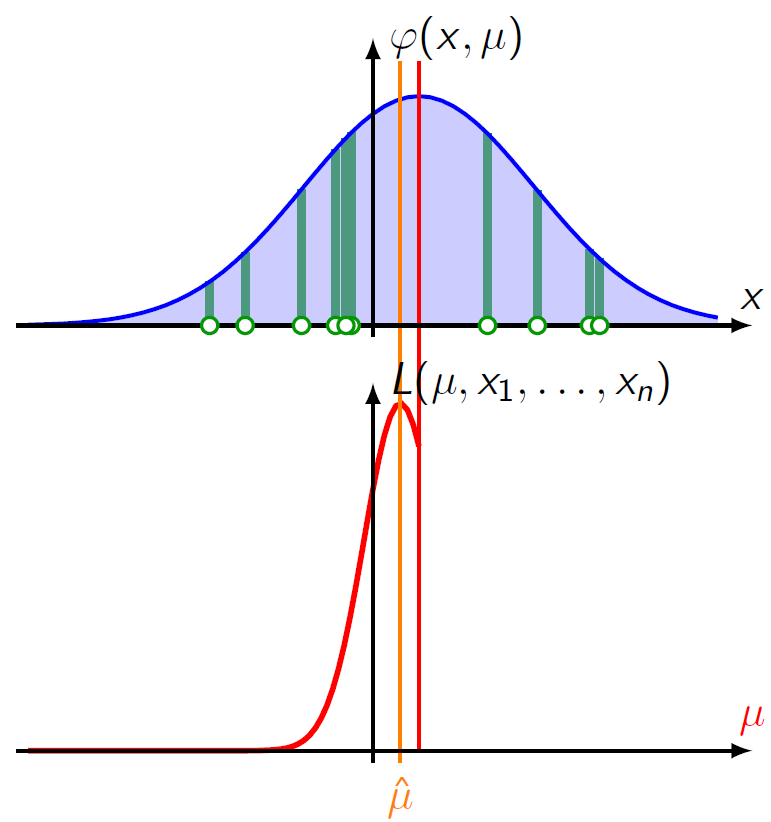
\includegraphics[width=\columnwidth]{images/likelihood.png} 
\end{minipage}
\hfill
\begin{minipage}{0.5\columnwidth}
    Bewerte Kandidaten $\crd{\mu}$ mit der Likelihood-Funktion 

    $$ L(\mu, x_1, ... x_n) = \cgn{\varphi(x_1, \mu)} \, ... \,  \cgn{\varphi(x_n, \mu)} $$
    $$ \text{ \textrightarrow\ } \cor{\hat{\mu}} = \mathrm{arg \, max}_{\substack{\mu}} L(\mu, x_1, ... x_n) $$
\end{minipage}

\vspace{0.2cm}

\myul{\textbf{Likelihood-Funktion}}
$$ L(\vartheta, x_1, ... x_n) = \varphi(\vartheta, x_1) \cdot \varphi(\vartheta, x_2) ... \varphi(\vartheta, x_n) $$
Wahrscheinlichkeit für die Werte $x_i$ 

\vspace{0.2cm}

\myul{\textbf{Prinzip}}
\vspace{0.1cm}

$\hat{\vartheta}(x_1, ..., x_n)$ maximiert  $L(\vartheta, x_1, ... x_n)$ (Maximum-Likelihood-Schätzer) \\
\textrightarrow\ Ableiten und Null setzen!


\example{Schätzung von $\bm{\mu}$}

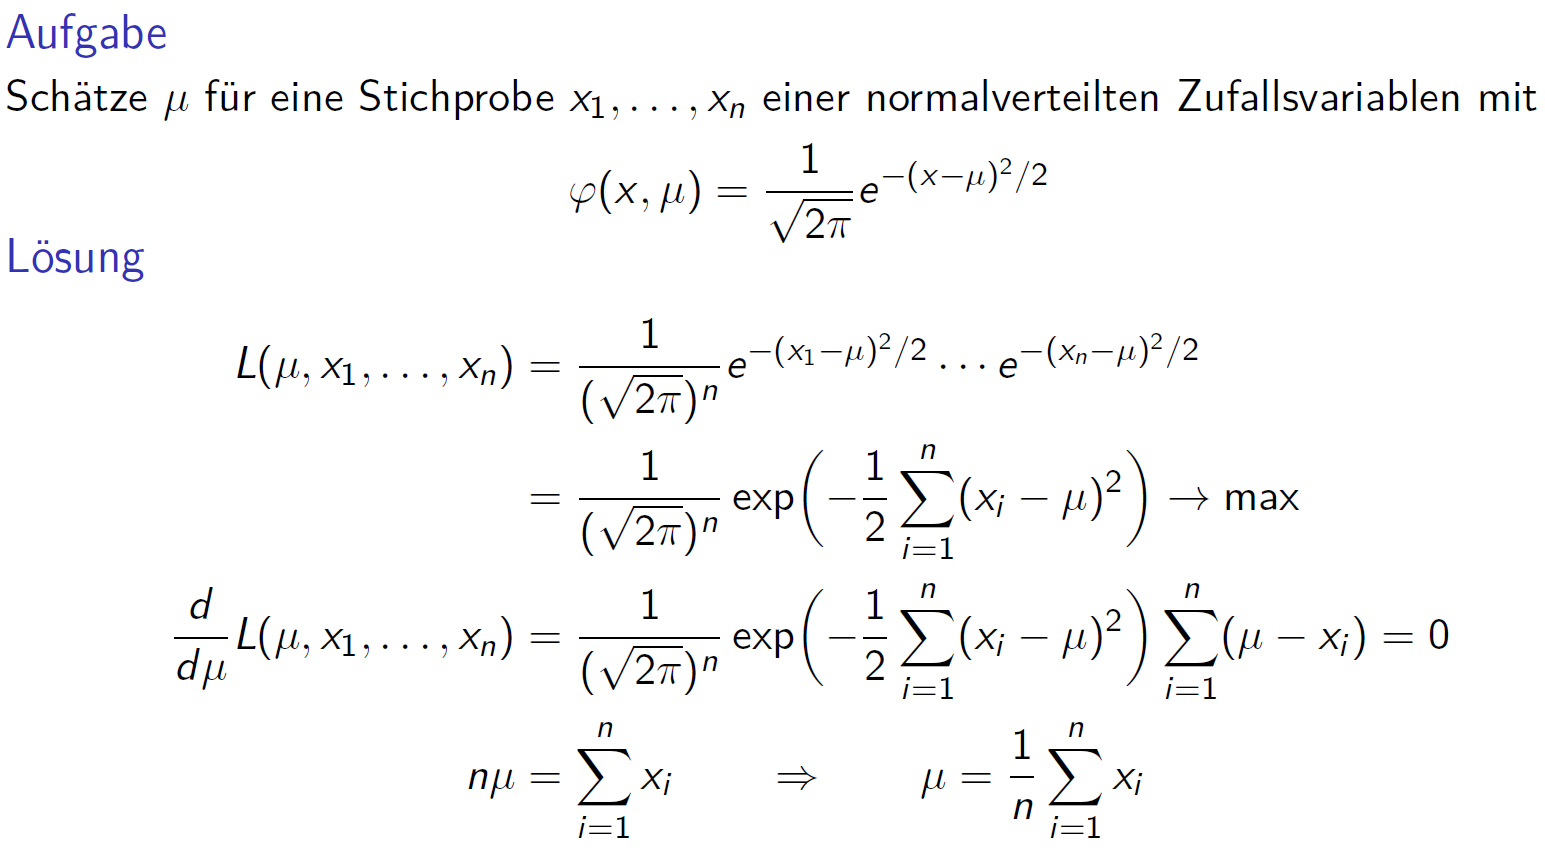
\includegraphics[width=\columnwidth]{images/likelihood_beispiel.png}


\subsection{Konfidenzintervall}

 $[\vartheta_-, \vartheta_+]$ heisst \textbf{Konfidenzintervall} zum (Vertrauens-)Niveau $1 - \alpha$ 

\vspace{0.2cm}

\myul{\textbf{Aufgabe:}}

\vspace{0.1cm}

Finde ein Intervall $[\vartheta_-, \vartheta_+]$, das den wahren Wert des Parameters mit Wahrscheinlichkeit $1 - \alpha$ enthält.

\vspace{0.2cm}

\begin{minipage}{0.4\columnwidth}
    \includegraphics[width=\columnwidth]{images/Konfidenzintervall}
\end{minipage}
\hfill
\begin{minipage}{0.55\columnwidth}
    \myul{\textbf{Lösung}}

    \vspace{0.1cm}

    \begin{itemize}
        \item  Verteilung von $\hat{\vartheta}$: \\
            Wahrscheinlichkeitsdichte $\varphi(\hat{\vartheta})$ und Verteilungsfunktion $F_{\hat{\vartheta}}$
        \item Finde $\vartheta$-Werte so, dass $1 - \alpha = F(\vartheta_+) - F(\vartheta_-)$
    \end{itemize}
\end{minipage}

\vspace{0.1cm}

{\small \textrightarrow\ Zweiseitig: $\frac{\alpha}{2}$ pro Seite \textrightarrow\ Quantil $1 - \frac{\alpha}{2}$ \quad (95\,\% \textrightarrow\ \textbf{0,975}, nicht 0,95)\par}


\subsection{Intervallschätzung}
\label{sec:intervallschaetzung}
\definecolor{qgn}{HTML}{2E8B3A}

\myul{\textbf{Aufgabe}}

\vspace{0.1cm}

Normalverteilte Stichprobe $X_1, \, \ldots, \, X_n$, \ $\hat{\mu} = \frac{1}{n} (X_1 + \ldots + X_n)$. \\
Finde ein Intervall, das $\mu$ (bzw. eine einzelne Messung $X$) mit Wahrscheinlichkeit 95\,\% enthält.

$$ \boxed{ \text{Intervall} = \text{Mitte} \pm \textcolor{qgn}{\text{Quantil}} \cdot \text{Breite} } $$

\begin{minipage}{0.37\columnwidth}
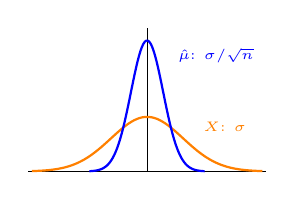
\begin{tikzpicture}
\begin{axis}[width=4.6cm, height=3.4cm, axis lines=middle, axis line style={-}, ticks=none,
             xmin=-3.3, xmax=3.3, ymin=0, ymax=1.05, clip=false]
  \addplot[orange, thick, samples=80, domain=-3.2:3.2] {0.4*exp(-x^2/2)};
  \addplot[blue, thick, samples=80, domain=-1.6:1.6] {0.96*exp(-x^2/(2*0.2))};
  \node[blue, font=\tiny, anchor=west] at (axis cs:0.6,0.85) {$\hat{\mu}$: $\sigma/\sqrt{n}$};
  \node[orange, font=\tiny, anchor=west] at (axis cs:1.3,0.33) {$X$: $\sigma$};
\end{axis}
\end{tikzpicture}
\end{minipage}
\hfill
\begin{minipage}{0.6\columnwidth}
\small
\textbf{Frage 1 \textrightarrow\ Breite} \\
Mittelwert $\mu$ gesucht \textrightarrow\ $\cbl{\sigma/\sqrt{n}}$ \\
einzelne Messung $X$ \textrightarrow\ $\cor{\sigma}$

\vspace{0.15cm}

\textbf{Frage 2 \textrightarrow\ Quantil} \\
$\sigma$ gegeben \textrightarrow\ $\textcolor{qgn}{z = 1.96}$ \\
$\hat{\sigma}$ aus Daten \textrightarrow\ $\textcolor{qgn}{t_+}$ \ ($k = n-1$, Spalte 0,975)
\end{minipage}

\vspace{0.2cm}

{\small
\renewcommand{\arraystretch}{2}
\begin{tabular}{@{}l l l@{}}
\toprule
 & \textbf{$\bm{\sigma}$ gegeben} & \textbf{$\bm{\hat{\sigma}}$ aus Daten} \\
\midrule
\textbf{Mittelwert $\bm{\mu}$} & $\hat{\mu} \pm \textcolor{qgn}{1.96} \cdot \cbl{\dfrac{\sigma}{\sqrt{n}}}$ & $\hat{\mu} \pm \textcolor{qgn}{t_+} \cdot \cbl{\dfrac{\hat{\sigma}}{\sqrt{n}}}$ \\
\textbf{einzelnes $\bm{X}$}    & $\mu \pm \textcolor{qgn}{1.96} \cdot \cor{\sigma}$ & $\hat{\mu} \pm \textcolor{qgn}{t_+} \cdot \cor{\hat{\sigma}}$ \\
\bottomrule
\end{tabular}
\par}

\vspace{0.1cm}

{\small \textrightarrow\ $\textcolor{qgn}{t_+}$: $t$-Tabelle (Abschnitt \ref{Quantilen der t-Verteilung}) \quad | \quad $\hat{\sigma}^2$ mit $\frac{1}{n-1}$ (Abschnitt \ref{sec:parameter-schaetzen})\par}
{\small \textrightarrow\ Warum $t$: $\dfrac{\hat{\mu} - \mu}{\hat{\sigma}/\sqrt{n}}$ bzw. $\dfrac{X - \hat{\mu}}{\hat{\sigma}}$ ist $t$-verteilt mit $k = n-1$\par}
{\small \textrightarrow\ $t$ = Normalverteilung mit dickeren Rändern, weil $\hat{\sigma}$ selbst unsicher ist\par}
{\small \textrightarrow\ $k = n-1$: die Abweichungen $x_i - \bar{x}$ summieren zu 0 \textrightarrow\ nur $n-1$ frei\par}

\vspace{0.1cm}

\definecolor{warnbg}{HTML}{FCEFEA}\definecolor{warnfr}{HTML}{A3341B}
\begin{tcolorbox}[colback=warnbg, colframe=warnfr, coltext=black, boxrule=0.4pt, arc=1pt, left=3pt, right=3pt, top=2pt, bottom=2pt]
\small
\textbf{Achtung} \\
\textrightarrow\ $\sigma^2$ gegeben \textrightarrow\ zuerst Wurzel ziehen \\
\textrightarrow\ $\hat{\sigma}$ aus Daten \textrightarrow\ HP Prime \textbf{sX} (nicht $\sigma$X) \\
\textrightarrow\ mehr Daten \textrightarrow\ $t_+$ kleiner; \ $k \to \infty$: $t_+ = 1.96$
\end{tcolorbox}
